\documentclass[twoside]{book}

% Packages required by doxygen
\usepackage{fixltx2e}
\usepackage{calc}
\usepackage{doxygen}
\usepackage[export]{adjustbox} % also loads graphicx
\usepackage{graphicx}
\usepackage[utf8]{inputenc}
\usepackage{makeidx}
\usepackage{multicol}
\usepackage{multirow}
\PassOptionsToPackage{warn}{textcomp}
\usepackage{textcomp}
\usepackage[nointegrals]{wasysym}
\usepackage[table]{xcolor}

% Font selection
\usepackage[T1]{fontenc}
\usepackage[scaled=.90]{helvet}
\usepackage{courier}
\usepackage{amssymb}
\usepackage{sectsty}
\renewcommand{\familydefault}{\sfdefault}
\allsectionsfont{%
  \fontseries{bc}\selectfont%
  \color{darkgray}%
}
\renewcommand{\DoxyLabelFont}{%
  \fontseries{bc}\selectfont%
  \color{darkgray}%
}
\newcommand{\+}{\discretionary{\mbox{\scriptsize$\hookleftarrow$}}{}{}}

% Page & text layout
\usepackage{geometry}
\geometry{%
  a4paper,%
  top=2.5cm,%
  bottom=2.5cm,%
  left=2.5cm,%
  right=2.5cm%
}
\tolerance=750
\hfuzz=15pt
\hbadness=750
\setlength{\emergencystretch}{15pt}
\setlength{\parindent}{0cm}
\setlength{\parskip}{0.2cm}
\makeatletter
\renewcommand{\paragraph}{%
  \@startsection{paragraph}{4}{0ex}{-1.0ex}{1.0ex}{%
    \normalfont\normalsize\bfseries\SS@parafont%
  }%
}
\renewcommand{\subparagraph}{%
  \@startsection{subparagraph}{5}{0ex}{-1.0ex}{1.0ex}{%
    \normalfont\normalsize\bfseries\SS@subparafont%
  }%
}
\makeatother

% Headers & footers
\usepackage{fancyhdr}
\pagestyle{fancyplain}
\fancyhead[LE]{\fancyplain{}{\bfseries\thepage}}
\fancyhead[CE]{\fancyplain{}{}}
\fancyhead[RE]{\fancyplain{}{\bfseries\leftmark}}
\fancyhead[LO]{\fancyplain{}{\bfseries\rightmark}}
\fancyhead[CO]{\fancyplain{}{}}
\fancyhead[RO]{\fancyplain{}{\bfseries\thepage}}
\fancyfoot[LE]{\fancyplain{}{}}
\fancyfoot[CE]{\fancyplain{}{}}
\fancyfoot[RE]{\fancyplain{}{\bfseries\scriptsize Generated on Mon Nov 16 2015 12\+:56\+:05 for My Project by Doxygen }}
\fancyfoot[LO]{\fancyplain{}{\bfseries\scriptsize Generated on Mon Nov 16 2015 12\+:56\+:05 for My Project by Doxygen }}
\fancyfoot[CO]{\fancyplain{}{}}
\fancyfoot[RO]{\fancyplain{}{}}
\renewcommand{\footrulewidth}{0.4pt}
\renewcommand{\chaptermark}[1]{%
  \markboth{#1}{}%
}
\renewcommand{\sectionmark}[1]{%
  \markright{\thesection\ #1}%
}

% Indices & bibliography
\usepackage{natbib}
\usepackage[titles]{tocloft}
\setcounter{tocdepth}{3}
\setcounter{secnumdepth}{5}
\makeindex

% Hyperlinks (required, but should be loaded last)
\usepackage{ifpdf}
\ifpdf
  \usepackage[pdftex,pagebackref=true]{hyperref}
\else
  \usepackage[ps2pdf,pagebackref=true]{hyperref}
\fi
\hypersetup{%
  colorlinks=true,%
  linkcolor=blue,%
  citecolor=blue,%
  unicode%
}

% Custom commands
\newcommand{\clearemptydoublepage}{%
  \newpage{\pagestyle{empty}\cleardoublepage}%
}


%===== C O N T E N T S =====

\begin{document}

% Titlepage & ToC
\hypersetup{pageanchor=false,
             bookmarks=true,
             bookmarksnumbered=true,
             pdfencoding=unicode
            }
\pagenumbering{roman}
\begin{titlepage}
\vspace*{7cm}
\begin{center}%
{\Large My Project }\\
\vspace*{1cm}
{\large Generated by Doxygen 1.8.10}\\
\vspace*{0.5cm}
{\small Mon Nov 16 2015 12:56:05}\\
\end{center}
\end{titlepage}
\clearemptydoublepage
\tableofcontents
\clearemptydoublepage
\pagenumbering{arabic}
\hypersetup{pageanchor=true}

%--- Begin generated contents ---
\chapter{Hierarchical Index}
\section{Class Hierarchy}
This inheritance list is sorted roughly, but not completely, alphabetically\+:\begin{DoxyCompactList}
\item \contentsline{section}{Customer}{\pageref{class_customer}}{}
\item \contentsline{section}{Queue.\+Node}{\pageref{class_queue_1_1_node}}{}
\item \contentsline{section}{Queue}{\pageref{class_queue}}{}
\item \contentsline{section}{Register}{\pageref{class_register}}{}
\item Runtime\+Exception\begin{DoxyCompactList}
\item \contentsline{section}{Queue.\+Empty\+Queue\+Exception}{\pageref{class_queue_1_1_empty_queue_exception}}{}
\end{DoxyCompactList}
\item \contentsline{section}{Simulation}{\pageref{class_simulation}}{}
\item \contentsline{section}{Simulator}{\pageref{class_simulator}}{}
\item \contentsline{section}{Store}{\pageref{class_store}}{}
\end{DoxyCompactList}

\chapter{Class Index}
\section{Class List}
Here are the classes, structs, unions and interfaces with brief descriptions\+:\begin{DoxyCompactList}
\item\contentsline{section}{\hyperlink{class_customer}{Customer} }{\pageref{class_customer}}{}
\item\contentsline{section}{\hyperlink{class_queue_1_1_empty_queue_exception}{Queue.\+Empty\+Queue\+Exception} }{\pageref{class_queue_1_1_empty_queue_exception}}{}
\item\contentsline{section}{\hyperlink{class_queue_1_1_node}{Queue.\+Node} }{\pageref{class_queue_1_1_node}}{}
\item\contentsline{section}{\hyperlink{class_queue}{Queue} }{\pageref{class_queue}}{}
\item\contentsline{section}{\hyperlink{class_register}{Register} }{\pageref{class_register}}{}
\item\contentsline{section}{\hyperlink{class_simulation}{Simulation} }{\pageref{class_simulation}}{}
\item\contentsline{section}{\hyperlink{class_simulator}{Simulator} }{\pageref{class_simulator}}{}
\item\contentsline{section}{\hyperlink{class_store}{Store} }{\pageref{class_store}}{}
\end{DoxyCompactList}

\chapter{Class Documentation}
\hypertarget{class_customer}{}\section{Customer Class Reference}
\label{class_customer}\index{Customer@{Customer}}
\subsection*{Public Member Functions}
\begin{DoxyCompactItemize}
\item 
\hyperlink{class_customer_a8ae55c351b09b5f5839ea5caea9971e5}{Customer} (int borntime, int groceries)
\item 
void \hyperlink{class_customer_a2b6d33ea417c8496fbb46e9aa0566c7d}{serve} ()
\item 
boolean \hyperlink{class_customer_a941cb1b5e2ed9d3d6f44cad0cb1a60a3}{is\+Done} (\hyperlink{class_customer}{Customer} c)
\item 
int \hyperlink{class_customer_a5a6a7257efe6835348f14334f6857fa0}{get\+Born\+Time} ()
\item 
int \hyperlink{class_customer_a205c4ccb6d3c6ae9902e0bb48cad9f5c}{get\+Groceries} ()
\item 
String \hyperlink{class_customer_ad2d375466bd51b83c89490333ab1b859}{to\+String} ()
\end{DoxyCompactItemize}


\subsection{Detailed Description}
Represents a customer in the store 
\begin{DoxyParams}{Parameters}
{\em borntime} & The timestep the customer arrived to the store \\
\hline
{\em groceries} & The number of groceries the customer has \\
\hline
\end{DoxyParams}


\subsection{Constructor \& Destructor Documentation}
\hypertarget{class_customer_a8ae55c351b09b5f5839ea5caea9971e5}{}\index{Customer@{Customer}!Customer@{Customer}}
\index{Customer@{Customer}!Customer@{Customer}}
\subsubsection[{Customer(int borntime, int groceries)}]{\setlength{\rightskip}{0pt plus 5cm}Customer.\+Customer (
\begin{DoxyParamCaption}
\item[{int}]{borntime, }
\item[{int}]{groceries}
\end{DoxyParamCaption}
)}\label{class_customer_a8ae55c351b09b5f5839ea5caea9971e5}
Creates a customer 
\begin{DoxyParams}{Parameters}
{\em borntime} & the given timestep \\
\hline
{\em grocieries} & the number of groceries \\
\hline
\end{DoxyParams}


\subsection{Member Function Documentation}
\hypertarget{class_customer_a5a6a7257efe6835348f14334f6857fa0}{}\index{Customer@{Customer}!get\+Born\+Time@{get\+Born\+Time}}
\index{get\+Born\+Time@{get\+Born\+Time}!Customer@{Customer}}
\subsubsection[{get\+Born\+Time()}]{\setlength{\rightskip}{0pt plus 5cm}int Customer.\+get\+Born\+Time (
\begin{DoxyParamCaption}
{}
\end{DoxyParamCaption}
)}\label{class_customer_a5a6a7257efe6835348f14334f6857fa0}
Checks which timestep the customer arrived to the store \begin{DoxyReturn}{Returns}
the timestep as an int 
\end{DoxyReturn}
\hypertarget{class_customer_a205c4ccb6d3c6ae9902e0bb48cad9f5c}{}\index{Customer@{Customer}!get\+Groceries@{get\+Groceries}}
\index{get\+Groceries@{get\+Groceries}!Customer@{Customer}}
\subsubsection[{get\+Groceries()}]{\setlength{\rightskip}{0pt plus 5cm}int Customer.\+get\+Groceries (
\begin{DoxyParamCaption}
{}
\end{DoxyParamCaption}
)}\label{class_customer_a205c4ccb6d3c6ae9902e0bb48cad9f5c}
Checks how many groceries a customer has \begin{DoxyReturn}{Returns}
the number of groceries 
\end{DoxyReturn}
\hypertarget{class_customer_a941cb1b5e2ed9d3d6f44cad0cb1a60a3}{}\index{Customer@{Customer}!is\+Done@{is\+Done}}
\index{is\+Done@{is\+Done}!Customer@{Customer}}
\subsubsection[{is\+Done(\+Customer c)}]{\setlength{\rightskip}{0pt plus 5cm}boolean Customer.\+is\+Done (
\begin{DoxyParamCaption}
\item[{{\bf Customer}}]{c}
\end{DoxyParamCaption}
)}\label{class_customer_a941cb1b5e2ed9d3d6f44cad0cb1a60a3}
Checks if a customer is done \begin{DoxyReturn}{Returns}
true if the customer is done, otherwise false 
\end{DoxyReturn}
\hypertarget{class_customer_a2b6d33ea417c8496fbb46e9aa0566c7d}{}\index{Customer@{Customer}!serve@{serve}}
\index{serve@{serve}!Customer@{Customer}}
\subsubsection[{serve()}]{\setlength{\rightskip}{0pt plus 5cm}void Customer.\+serve (
\begin{DoxyParamCaption}
{}
\end{DoxyParamCaption}
)}\label{class_customer_a2b6d33ea417c8496fbb46e9aa0566c7d}
\hyperlink{class_register}{Register} one of the customers groceries \hypertarget{class_customer_ad2d375466bd51b83c89490333ab1b859}{}\index{Customer@{Customer}!to\+String@{to\+String}}
\index{to\+String@{to\+String}!Customer@{Customer}}
\subsubsection[{to\+String()}]{\setlength{\rightskip}{0pt plus 5cm}String Customer.\+to\+String (
\begin{DoxyParamCaption}
{}
\end{DoxyParamCaption}
)}\label{class_customer_ad2d375466bd51b83c89490333ab1b859}
Prints a customer out as a string \begin{DoxyReturn}{Returns}
a string 
\end{DoxyReturn}


The documentation for this class was generated from the following file\+:\begin{DoxyCompactItemize}
\item 
Customer.\+java\end{DoxyCompactItemize}

\hypertarget{class_queue_1_1_empty_queue_exception}{}\section{Queue.\+Empty\+Queue\+Exception Class Reference}
\label{class_queue_1_1_empty_queue_exception}\index{Queue.\+Empty\+Queue\+Exception@{Queue.\+Empty\+Queue\+Exception}}
Inheritance diagram for Queue.\+Empty\+Queue\+Exception\+:\begin{figure}[H]
\begin{center}
\leavevmode
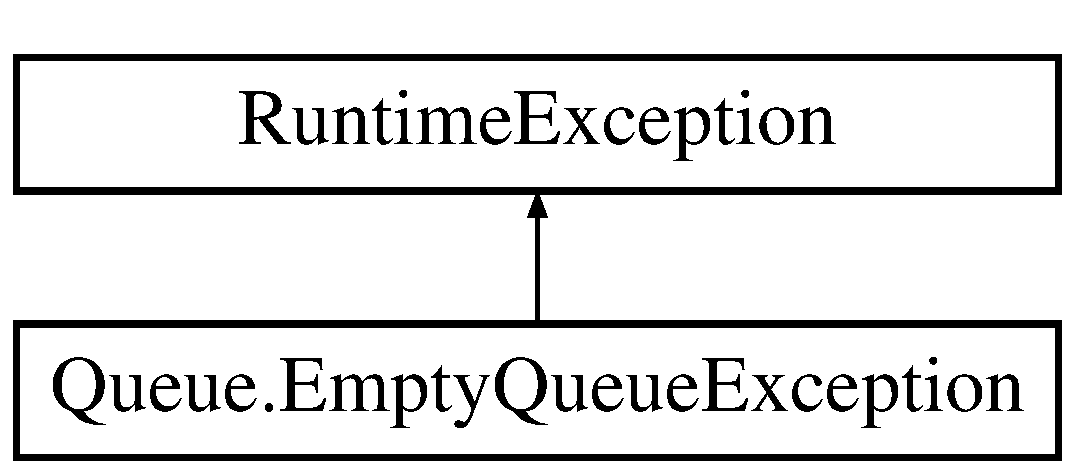
\includegraphics[height=2.000000cm]{class_queue_1_1_empty_queue_exception}
\end{center}
\end{figure}


\subsection{Detailed Description}
Creates an exeption for when the queue is empty 

The documentation for this class was generated from the following file\+:\begin{DoxyCompactItemize}
\item 
Queue.\+java\end{DoxyCompactItemize}

\hypertarget{class_queue_1_1_node}{}\section{Queue.\+Node Class Reference}
\label{class_queue_1_1_node}\index{Queue.\+Node@{Queue.\+Node}}
\subsection*{Public Attributes}
\begin{DoxyCompactItemize}
\item 
\hypertarget{class_queue_1_1_node_a2f6751fb2cfb71f9fa38582d2fcbeacc}{}\hyperlink{class_customer}{Customer} {\bfseries elem}\label{class_queue_1_1_node_a2f6751fb2cfb71f9fa38582d2fcbeacc}

\item 
\hypertarget{class_queue_1_1_node_a285b619a2d8165b0cd4feb283587164e}{}\hyperlink{class_queue_1_1_node}{Node} {\bfseries next}\label{class_queue_1_1_node_a285b619a2d8165b0cd4feb283587164e}

\end{DoxyCompactItemize}


\subsection{Detailed Description}
Represents a node in the queue 
\begin{DoxyParams}{Parameters}
{\em elem} & A customer in the queue \\
\hline
{\em next} & The next node in the queue \\
\hline
\end{DoxyParams}


The documentation for this class was generated from the following file\+:\begin{DoxyCompactItemize}
\item 
Queue.\+java\end{DoxyCompactItemize}

\hypertarget{class_queue}{}\section{Queue Class Reference}
\label{class_queue}\index{Queue@{Queue}}
\subsection*{Classes}
\begin{DoxyCompactItemize}
\item 
class \hyperlink{class_queue_1_1_empty_queue_exception}{Empty\+Queue\+Exception}
\item 
class \hyperlink{class_queue_1_1_node}{Node}
\end{DoxyCompactItemize}
\subsection*{Public Member Functions}
\begin{DoxyCompactItemize}
\item 
\hyperlink{class_queue_a42f2b12b7394e3005936c51f4f63ba41}{Queue} ()
\item 
boolean \hyperlink{class_queue_a9f7bee80c0f6221d577101879c617767}{is\+Empty} ()
\item 
int \hyperlink{class_queue_afdde374966974e3ac5fdc31d399f57f1}{length} ()
\item 
void \hyperlink{class_queue_aa6e1e6447ac35a97b0d885707be2f28f}{enqueue} (\hyperlink{class_customer}{Customer} elem)
\item 
\hyperlink{class_customer}{Customer} \hyperlink{class_queue_a3e352146ffd17e0fc870baa25cfba0b5}{dequeue} ()
\item 
\hyperlink{class_customer}{Customer} \hyperlink{class_queue_a05348ffe9ad100823cd0518651ff4e83}{first} ()
\item 
String \hyperlink{class_queue_a77c01ab03058b6d9707d29a4d3321693}{to\+String} ()
\end{DoxyCompactItemize}


\subsection{Detailed Description}
Represents a queue at a register in the store 
\begin{DoxyParams}{Parameters}
{\em length} & The length of the queue \\
\hline
{\em first} & The first node containing the first element in the queue \\
\hline
{\em last} & The last node containing the last element in the queue \\
\hline
\end{DoxyParams}


\subsection{Constructor \& Destructor Documentation}
\hypertarget{class_queue_a42f2b12b7394e3005936c51f4f63ba41}{}\index{Queue@{Queue}!Queue@{Queue}}
\index{Queue@{Queue}!Queue@{Queue}}
\subsubsection[{Queue()}]{\setlength{\rightskip}{0pt plus 5cm}Queue.\+Queue (
\begin{DoxyParamCaption}
{}
\end{DoxyParamCaption}
)}\label{class_queue_a42f2b12b7394e3005936c51f4f63ba41}
Creates a new queue 

\subsection{Member Function Documentation}
\hypertarget{class_queue_a3e352146ffd17e0fc870baa25cfba0b5}{}\index{Queue@{Queue}!dequeue@{dequeue}}
\index{dequeue@{dequeue}!Queue@{Queue}}
\subsubsection[{dequeue()}]{\setlength{\rightskip}{0pt plus 5cm}{\bf Customer} Queue.\+dequeue (
\begin{DoxyParamCaption}
{}
\end{DoxyParamCaption}
)}\label{class_queue_a3e352146ffd17e0fc870baa25cfba0b5}
Removes the first customer in the queue \begin{DoxyReturn}{Returns}
the removed customer 
\end{DoxyReturn}
\hypertarget{class_queue_aa6e1e6447ac35a97b0d885707be2f28f}{}\index{Queue@{Queue}!enqueue@{enqueue}}
\index{enqueue@{enqueue}!Queue@{Queue}}
\subsubsection[{enqueue(\+Customer elem)}]{\setlength{\rightskip}{0pt plus 5cm}void Queue.\+enqueue (
\begin{DoxyParamCaption}
\item[{{\bf Customer}}]{elem}
\end{DoxyParamCaption}
)}\label{class_queue_aa6e1e6447ac35a97b0d885707be2f28f}
Enqueues a customer last in the queue 
\begin{DoxyParams}{Parameters}
{\em elem} & a customer to be enqueued \\
\hline
\end{DoxyParams}
\hypertarget{class_queue_a05348ffe9ad100823cd0518651ff4e83}{}\index{Queue@{Queue}!first@{first}}
\index{first@{first}!Queue@{Queue}}
\subsubsection[{first()}]{\setlength{\rightskip}{0pt plus 5cm}{\bf Customer} Queue.\+first (
\begin{DoxyParamCaption}
{}
\end{DoxyParamCaption}
)}\label{class_queue_a05348ffe9ad100823cd0518651ff4e83}
Takes the first customer in the queue \begin{DoxyReturn}{Returns}
the first customer 
\end{DoxyReturn}
\hypertarget{class_queue_a9f7bee80c0f6221d577101879c617767}{}\index{Queue@{Queue}!is\+Empty@{is\+Empty}}
\index{is\+Empty@{is\+Empty}!Queue@{Queue}}
\subsubsection[{is\+Empty()}]{\setlength{\rightskip}{0pt plus 5cm}boolean Queue.\+is\+Empty (
\begin{DoxyParamCaption}
{}
\end{DoxyParamCaption}
)}\label{class_queue_a9f7bee80c0f6221d577101879c617767}
Checks if a queue is empty \begin{DoxyReturn}{Returns}
true if the queue is empty 
\end{DoxyReturn}
\hypertarget{class_queue_afdde374966974e3ac5fdc31d399f57f1}{}\index{Queue@{Queue}!length@{length}}
\index{length@{length}!Queue@{Queue}}
\subsubsection[{length()}]{\setlength{\rightskip}{0pt plus 5cm}int Queue.\+length (
\begin{DoxyParamCaption}
{}
\end{DoxyParamCaption}
)}\label{class_queue_afdde374966974e3ac5fdc31d399f57f1}
Checks the length of a queue \begin{DoxyReturn}{Returns}
the length as an int 
\end{DoxyReturn}
\hypertarget{class_queue_a77c01ab03058b6d9707d29a4d3321693}{}\index{Queue@{Queue}!to\+String@{to\+String}}
\index{to\+String@{to\+String}!Queue@{Queue}}
\subsubsection[{to\+String()}]{\setlength{\rightskip}{0pt plus 5cm}String Queue.\+to\+String (
\begin{DoxyParamCaption}
{}
\end{DoxyParamCaption}
)}\label{class_queue_a77c01ab03058b6d9707d29a4d3321693}
Prints a queue as a string \begin{DoxyReturn}{Returns}
a string 
\end{DoxyReturn}


The documentation for this class was generated from the following file\+:\begin{DoxyCompactItemize}
\item 
Queue.\+java\end{DoxyCompactItemize}

\hypertarget{class_register}{}\section{Register Class Reference}
\label{class_register}\index{Register@{Register}}
\subsection*{Public Member Functions}
\begin{DoxyCompactItemize}
\item 
\hyperlink{class_register_af15631d2edc3c9b87166f923b3d3a00f}{Register} ()
\item 
\hyperlink{class_register_a938cbf78ca6f8b7d738a2e6aa4b2ba42}{Register} (boolean \+\_\+open)
\item 
void \hyperlink{class_register_a9ed3f3799b5ea459d6df53f82b54e69f}{add\+To\+Queue} (\hyperlink{class_customer}{Customer} c)
\item 
\hyperlink{class_queue}{Queue} \hyperlink{class_register_a6f712d705f87c1a1d0bb9acd054bb453}{get\+Queue} ()
\item 
void \hyperlink{class_register_ac02a67e31b492873afbbc5ce2840d7fb}{open} ()
\item 
void \hyperlink{class_register_a6ff4bf08b8934138ae25ebdbdaa9a968}{close} ()
\item 
boolean \hyperlink{class_register_a892ac0d31549027d495948c82ff3ae7a}{is\+Open} ()
\item 
void \hyperlink{class_register_a71c5705fbba0bf88661cf3e7dd3b10d1}{step} ()
\item 
boolean \hyperlink{class_register_ae7c8276901821f6e866472afa54441a7}{has\+Customers} ()
\item 
boolean \hyperlink{class_register_a5feae9eebb986ff4798ba79a5b1f0c0a}{current\+Customer\+Is\+Done} ()
\item 
\hyperlink{class_customer}{Customer} \hyperlink{class_register_a09213fdfd15a583e5c6fe0bbe8505da3}{remove\+Current\+Customer} ()
\item 
int \hyperlink{class_register_a447023dcde7ef511a8222805114017e5}{get\+Queue\+Length} ()
\item 
String \hyperlink{class_register_ab27bc35d9b9514d42378b23193bf5dee}{to\+String} ()
\end{DoxyCompactItemize}


\subsection{Detailed Description}
Represents a register in a store 
\begin{DoxyParams}{Parameters}
{\em open} & A boolean representing if the register is open \\
\hline
{\em queue} & The register´s queue of customers \\
\hline
\end{DoxyParams}


\subsection{Constructor \& Destructor Documentation}
\hypertarget{class_register_af15631d2edc3c9b87166f923b3d3a00f}{}\index{Register@{Register}!Register@{Register}}
\index{Register@{Register}!Register@{Register}}
\subsubsection[{Register()}]{\setlength{\rightskip}{0pt plus 5cm}Register.\+Register (
\begin{DoxyParamCaption}
{}
\end{DoxyParamCaption}
)}\label{class_register_af15631d2edc3c9b87166f923b3d3a00f}
Creates a register \hypertarget{class_register_a938cbf78ca6f8b7d738a2e6aa4b2ba42}{}\index{Register@{Register}!Register@{Register}}
\index{Register@{Register}!Register@{Register}}
\subsubsection[{Register(boolean \+\_\+open)}]{\setlength{\rightskip}{0pt plus 5cm}Register.\+Register (
\begin{DoxyParamCaption}
\item[{boolean}]{\+\_\+open}
\end{DoxyParamCaption}
)}\label{class_register_a938cbf78ca6f8b7d738a2e6aa4b2ba42}
Creates an open register 

\subsection{Member Function Documentation}
\hypertarget{class_register_a9ed3f3799b5ea459d6df53f82b54e69f}{}\index{Register@{Register}!add\+To\+Queue@{add\+To\+Queue}}
\index{add\+To\+Queue@{add\+To\+Queue}!Register@{Register}}
\subsubsection[{add\+To\+Queue(\+Customer c)}]{\setlength{\rightskip}{0pt plus 5cm}void Register.\+add\+To\+Queue (
\begin{DoxyParamCaption}
\item[{{\bf Customer}}]{c}
\end{DoxyParamCaption}
)}\label{class_register_a9ed3f3799b5ea459d6df53f82b54e69f}
Adds a customer last in the registers queue 
\begin{DoxyParams}{Parameters}
{\em c} & the customer to be queued \\
\hline
\end{DoxyParams}
\hypertarget{class_register_a6ff4bf08b8934138ae25ebdbdaa9a968}{}\index{Register@{Register}!close@{close}}
\index{close@{close}!Register@{Register}}
\subsubsection[{close()}]{\setlength{\rightskip}{0pt plus 5cm}void Register.\+close (
\begin{DoxyParamCaption}
{}
\end{DoxyParamCaption}
)}\label{class_register_a6ff4bf08b8934138ae25ebdbdaa9a968}
Closes a register \hypertarget{class_register_a5feae9eebb986ff4798ba79a5b1f0c0a}{}\index{Register@{Register}!current\+Customer\+Is\+Done@{current\+Customer\+Is\+Done}}
\index{current\+Customer\+Is\+Done@{current\+Customer\+Is\+Done}!Register@{Register}}
\subsubsection[{current\+Customer\+Is\+Done()}]{\setlength{\rightskip}{0pt plus 5cm}boolean Register.\+current\+Customer\+Is\+Done (
\begin{DoxyParamCaption}
{}
\end{DoxyParamCaption}
)}\label{class_register_a5feae9eebb986ff4798ba79a5b1f0c0a}
Checks if the first customer in the queue is finished \begin{DoxyReturn}{Returns}
true if the customer is done, otherwise false 
\end{DoxyReturn}
\hypertarget{class_register_a6f712d705f87c1a1d0bb9acd054bb453}{}\index{Register@{Register}!get\+Queue@{get\+Queue}}
\index{get\+Queue@{get\+Queue}!Register@{Register}}
\subsubsection[{get\+Queue()}]{\setlength{\rightskip}{0pt plus 5cm}{\bf Queue} Register.\+get\+Queue (
\begin{DoxyParamCaption}
{}
\end{DoxyParamCaption}
)}\label{class_register_a6f712d705f87c1a1d0bb9acd054bb453}
Takes a queue \begin{DoxyReturn}{Returns}
a queue 
\end{DoxyReturn}
\hypertarget{class_register_a447023dcde7ef511a8222805114017e5}{}\index{Register@{Register}!get\+Queue\+Length@{get\+Queue\+Length}}
\index{get\+Queue\+Length@{get\+Queue\+Length}!Register@{Register}}
\subsubsection[{get\+Queue\+Length()}]{\setlength{\rightskip}{0pt plus 5cm}int Register.\+get\+Queue\+Length (
\begin{DoxyParamCaption}
{}
\end{DoxyParamCaption}
)}\label{class_register_a447023dcde7ef511a8222805114017e5}
Checks the length of a registers queue \begin{DoxyReturn}{Returns}
the length of a queue 
\end{DoxyReturn}
\hypertarget{class_register_ae7c8276901821f6e866472afa54441a7}{}\index{Register@{Register}!has\+Customers@{has\+Customers}}
\index{has\+Customers@{has\+Customers}!Register@{Register}}
\subsubsection[{has\+Customers()}]{\setlength{\rightskip}{0pt plus 5cm}boolean Register.\+has\+Customers (
\begin{DoxyParamCaption}
{}
\end{DoxyParamCaption}
)}\label{class_register_ae7c8276901821f6e866472afa54441a7}
Checks if a register has any customers in line \begin{DoxyReturn}{Returns}
true if the queue is empty, otherwise false 
\end{DoxyReturn}
\hypertarget{class_register_a892ac0d31549027d495948c82ff3ae7a}{}\index{Register@{Register}!is\+Open@{is\+Open}}
\index{is\+Open@{is\+Open}!Register@{Register}}
\subsubsection[{is\+Open()}]{\setlength{\rightskip}{0pt plus 5cm}boolean Register.\+is\+Open (
\begin{DoxyParamCaption}
{}
\end{DoxyParamCaption}
)}\label{class_register_a892ac0d31549027d495948c82ff3ae7a}
Checks if a register is open \begin{DoxyReturn}{Returns}
true if the register is open, otherwise false 
\end{DoxyReturn}
\hypertarget{class_register_ac02a67e31b492873afbbc5ce2840d7fb}{}\index{Register@{Register}!open@{open}}
\index{open@{open}!Register@{Register}}
\subsubsection[{open()}]{\setlength{\rightskip}{0pt plus 5cm}void Register.\+open (
\begin{DoxyParamCaption}
{}
\end{DoxyParamCaption}
)}\label{class_register_ac02a67e31b492873afbbc5ce2840d7fb}
Opens a register \hypertarget{class_register_a09213fdfd15a583e5c6fe0bbe8505da3}{}\index{Register@{Register}!remove\+Current\+Customer@{remove\+Current\+Customer}}
\index{remove\+Current\+Customer@{remove\+Current\+Customer}!Register@{Register}}
\subsubsection[{remove\+Current\+Customer()}]{\setlength{\rightskip}{0pt plus 5cm}{\bf Customer} Register.\+remove\+Current\+Customer (
\begin{DoxyParamCaption}
{}
\end{DoxyParamCaption}
)}\label{class_register_a09213fdfd15a583e5c6fe0bbe8505da3}
Removes the first customer in the queue \begin{DoxyReturn}{Returns}
the removed customer 
\end{DoxyReturn}
\hypertarget{class_register_a71c5705fbba0bf88661cf3e7dd3b10d1}{}\index{Register@{Register}!step@{step}}
\index{step@{step}!Register@{Register}}
\subsubsection[{step()}]{\setlength{\rightskip}{0pt plus 5cm}void Register.\+step (
\begin{DoxyParamCaption}
{}
\end{DoxyParamCaption}
)}\label{class_register_a71c5705fbba0bf88661cf3e7dd3b10d1}
Serves the first customer in the queue \hypertarget{class_register_ab27bc35d9b9514d42378b23193bf5dee}{}\index{Register@{Register}!to\+String@{to\+String}}
\index{to\+String@{to\+String}!Register@{Register}}
\subsubsection[{to\+String()}]{\setlength{\rightskip}{0pt plus 5cm}String Register.\+to\+String (
\begin{DoxyParamCaption}
{}
\end{DoxyParamCaption}
)}\label{class_register_ab27bc35d9b9514d42378b23193bf5dee}
Prints a register as a string \begin{DoxyReturn}{Returns}
a string 
\end{DoxyReturn}


The documentation for this class was generated from the following file\+:\begin{DoxyCompactItemize}
\item 
Register.\+java\end{DoxyCompactItemize}

\hypertarget{class_simulation}{}\section{Simulation Class Reference}
\label{class_simulation}\index{Simulation@{Simulation}}
\subsection*{Public Member Functions}
\begin{DoxyCompactItemize}
\item 
\hyperlink{class_simulation_aa24c4314fd1e140a1b9ad5feb06c6fb0}{Simulation} ()
\item 
\hyperlink{class_simulation_aae94561923d7826c754567121f6b1042}{Simulation} (int \+\_\+intensity, int \+\_\+max\+Groceries, double \+\_\+threshold\+For\+New\+Register, int \+\_\+number\+Of\+Registers)
\item 
int \hyperlink{class_simulation_a1f4d6be58ea9284bbafac04ff9cff2f3}{get\+Time} ()
\item 
int \hyperlink{class_simulation_ab743aabfae74983b6e475caadfc5072f}{get\+Intensity} ()
\item 
int \hyperlink{class_simulation_a60e2eec59d7d04570369d014d2c585c3}{get\+Max\+Groceries} ()
\item 
double \hyperlink{class_simulation_a6685cc83b16bcac230972576a424b742}{get\+Threshold\+For\+New\+Register} ()
\item 
double \hyperlink{class_simulation_a8e21a8270cb67b355d68dcd7b61c3aac}{get\+Average\+Wait\+Time} ()
\item 
int \hyperlink{class_simulation_a98b45946461dbf1f68f4790036b67ac3}{get\+Number\+Of\+Customers\+Served} ()
\item 
int \hyperlink{class_simulation_ac44576077cf39f3c772df0b0f956a460}{get\+Longest\+Wait\+Time} ()
\item 
void \hyperlink{class_simulation_a191a1c3bdd167494288a49206657090c}{step} ()
\item 
String \hyperlink{class_simulation_a62bc9c7d0357063026acf3682b362552}{to\+String} ()
\end{DoxyCompactItemize}
\subsection*{Static Public Member Functions}
\begin{DoxyCompactItemize}
\item 
\hypertarget{class_simulation_a9696222d4b2febd4a35411157f99957f}{}static void {\bfseries main} (String args\mbox{[}$\,$\mbox{]})\label{class_simulation_a9696222d4b2febd4a35411157f99957f}

\end{DoxyCompactItemize}


\subsection{Detailed Description}
Keeps track of the time and all statistics, determines when new customer arrives and when to open new registers. 
\begin{DoxyParams}{Parameters}
{\em store} & the store to be simulated \\
\hline
{\em time} & the number of timesteps since the simulation started \\
\hline
{\em intensity} & the probability there will arrive a new customer at every timestep \\
\hline
{\em max\+Groceries} & the maximum amount of groceries a customer can have \\
\hline
{\em threshold\+For\+New\+Register} & at what avarage length a new register should open \\
\hline
{\em average\+Wait\+Time} & the average wait time in the store \\
\hline
{\em number\+Of\+Customers\+Served} & the number of customer already served \\
\hline
{\em longest\+Wait\+Time} & the longest wait time in the store \\
\hline
{\em total\+Wait\+Time} & the total wait time for all customers in the store \\
\hline
\end{DoxyParams}


\subsection{Constructor \& Destructor Documentation}
\hypertarget{class_simulation_aa24c4314fd1e140a1b9ad5feb06c6fb0}{}\index{Simulation@{Simulation}!Simulation@{Simulation}}
\index{Simulation@{Simulation}!Simulation@{Simulation}}
\subsubsection[{Simulation()}]{\setlength{\rightskip}{0pt plus 5cm}Simulation.\+Simulation (
\begin{DoxyParamCaption}
{}
\end{DoxyParamCaption}
)}\label{class_simulation_aa24c4314fd1e140a1b9ad5feb06c6fb0}
Creates a simulation \hypertarget{class_simulation_aae94561923d7826c754567121f6b1042}{}\index{Simulation@{Simulation}!Simulation@{Simulation}}
\index{Simulation@{Simulation}!Simulation@{Simulation}}
\subsubsection[{Simulation(int \+\_\+intensity, int \+\_\+max\+Groceries, double \+\_\+threshold\+For\+New\+Register, int \+\_\+number\+Of\+Registers)}]{\setlength{\rightskip}{0pt plus 5cm}Simulation.\+Simulation (
\begin{DoxyParamCaption}
\item[{int}]{\+\_\+intensity, }
\item[{int}]{\+\_\+max\+Groceries, }
\item[{double}]{\+\_\+threshold\+For\+New\+Register, }
\item[{int}]{\+\_\+number\+Of\+Registers}
\end{DoxyParamCaption}
)}\label{class_simulation_aae94561923d7826c754567121f6b1042}
Creates a simulation with given parameters 
\begin{DoxyParams}{Parameters}
{\em \+\_\+intensity} & \\
\hline
{\em \+\_\+max\+Groceries} & the maximum groceries a customer can have \\
\hline
{\em \+\_\+threshold\+For\+New\+Register} & when to open new registers \\
\hline
{\em \+\_\+number\+Of\+Registers} & the number of registers \\
\hline
\end{DoxyParams}


\subsection{Member Function Documentation}
\hypertarget{class_simulation_a8e21a8270cb67b355d68dcd7b61c3aac}{}\index{Simulation@{Simulation}!get\+Average\+Wait\+Time@{get\+Average\+Wait\+Time}}
\index{get\+Average\+Wait\+Time@{get\+Average\+Wait\+Time}!Simulation@{Simulation}}
\subsubsection[{get\+Average\+Wait\+Time()}]{\setlength{\rightskip}{0pt plus 5cm}double Simulation.\+get\+Average\+Wait\+Time (
\begin{DoxyParamCaption}
{}
\end{DoxyParamCaption}
)}\label{class_simulation_a8e21a8270cb67b355d68dcd7b61c3aac}
Checks the average waittime in the store \begin{DoxyReturn}{Returns}
the average waittime 
\end{DoxyReturn}
\hypertarget{class_simulation_ab743aabfae74983b6e475caadfc5072f}{}\index{Simulation@{Simulation}!get\+Intensity@{get\+Intensity}}
\index{get\+Intensity@{get\+Intensity}!Simulation@{Simulation}}
\subsubsection[{get\+Intensity()}]{\setlength{\rightskip}{0pt plus 5cm}int Simulation.\+get\+Intensity (
\begin{DoxyParamCaption}
{}
\end{DoxyParamCaption}
)}\label{class_simulation_ab743aabfae74983b6e475caadfc5072f}
Checks the probability there will arrive a new customer at every timestep \begin{DoxyReturn}{Returns}
the probability in procent 
\end{DoxyReturn}
\hypertarget{class_simulation_ac44576077cf39f3c772df0b0f956a460}{}\index{Simulation@{Simulation}!get\+Longest\+Wait\+Time@{get\+Longest\+Wait\+Time}}
\index{get\+Longest\+Wait\+Time@{get\+Longest\+Wait\+Time}!Simulation@{Simulation}}
\subsubsection[{get\+Longest\+Wait\+Time()}]{\setlength{\rightskip}{0pt plus 5cm}int Simulation.\+get\+Longest\+Wait\+Time (
\begin{DoxyParamCaption}
{}
\end{DoxyParamCaption}
)}\label{class_simulation_ac44576077cf39f3c772df0b0f956a460}
Checks the longest waittime in the store \begin{DoxyReturn}{Returns}
the longest waittime 
\end{DoxyReturn}
\hypertarget{class_simulation_a60e2eec59d7d04570369d014d2c585c3}{}\index{Simulation@{Simulation}!get\+Max\+Groceries@{get\+Max\+Groceries}}
\index{get\+Max\+Groceries@{get\+Max\+Groceries}!Simulation@{Simulation}}
\subsubsection[{get\+Max\+Groceries()}]{\setlength{\rightskip}{0pt plus 5cm}int Simulation.\+get\+Max\+Groceries (
\begin{DoxyParamCaption}
{}
\end{DoxyParamCaption}
)}\label{class_simulation_a60e2eec59d7d04570369d014d2c585c3}
Checks the max amount of groceries a customer can have \begin{DoxyReturn}{Returns}
the maximum amount 
\end{DoxyReturn}
\hypertarget{class_simulation_a98b45946461dbf1f68f4790036b67ac3}{}\index{Simulation@{Simulation}!get\+Number\+Of\+Customers\+Served@{get\+Number\+Of\+Customers\+Served}}
\index{get\+Number\+Of\+Customers\+Served@{get\+Number\+Of\+Customers\+Served}!Simulation@{Simulation}}
\subsubsection[{get\+Number\+Of\+Customers\+Served()}]{\setlength{\rightskip}{0pt plus 5cm}int Simulation.\+get\+Number\+Of\+Customers\+Served (
\begin{DoxyParamCaption}
{}
\end{DoxyParamCaption}
)}\label{class_simulation_a98b45946461dbf1f68f4790036b67ac3}
Checks how many customer that has been served \begin{DoxyReturn}{Returns}
the number of customers been served 
\end{DoxyReturn}
\hypertarget{class_simulation_a6685cc83b16bcac230972576a424b742}{}\index{Simulation@{Simulation}!get\+Threshold\+For\+New\+Register@{get\+Threshold\+For\+New\+Register}}
\index{get\+Threshold\+For\+New\+Register@{get\+Threshold\+For\+New\+Register}!Simulation@{Simulation}}
\subsubsection[{get\+Threshold\+For\+New\+Register()}]{\setlength{\rightskip}{0pt plus 5cm}double Simulation.\+get\+Threshold\+For\+New\+Register (
\begin{DoxyParamCaption}
{}
\end{DoxyParamCaption}
)}\label{class_simulation_a6685cc83b16bcac230972576a424b742}
Checks at what average length a new register should open \begin{DoxyReturn}{Returns}
the average length as a double 
\end{DoxyReturn}
\hypertarget{class_simulation_a1f4d6be58ea9284bbafac04ff9cff2f3}{}\index{Simulation@{Simulation}!get\+Time@{get\+Time}}
\index{get\+Time@{get\+Time}!Simulation@{Simulation}}
\subsubsection[{get\+Time()}]{\setlength{\rightskip}{0pt plus 5cm}int Simulation.\+get\+Time (
\begin{DoxyParamCaption}
{}
\end{DoxyParamCaption}
)}\label{class_simulation_a1f4d6be58ea9284bbafac04ff9cff2f3}
Checks how many timesteps it has been since the simulation started \begin{DoxyReturn}{Returns}
the number of timesteps 
\end{DoxyReturn}
\hypertarget{class_simulation_a191a1c3bdd167494288a49206657090c}{}\index{Simulation@{Simulation}!step@{step}}
\index{step@{step}!Simulation@{Simulation}}
\subsubsection[{step()}]{\setlength{\rightskip}{0pt plus 5cm}void Simulation.\+step (
\begin{DoxyParamCaption}
{}
\end{DoxyParamCaption}
)}\label{class_simulation_a191a1c3bdd167494288a49206657090c}
Steps the time in the store one step and serves the first customer in every queue \hypertarget{class_simulation_a62bc9c7d0357063026acf3682b362552}{}\index{Simulation@{Simulation}!to\+String@{to\+String}}
\index{to\+String@{to\+String}!Simulation@{Simulation}}
\subsubsection[{to\+String()}]{\setlength{\rightskip}{0pt plus 5cm}String Simulation.\+to\+String (
\begin{DoxyParamCaption}
{}
\end{DoxyParamCaption}
)}\label{class_simulation_a62bc9c7d0357063026acf3682b362552}
Prints the simulation out as a string \begin{DoxyReturn}{Returns}
a string 
\end{DoxyReturn}


The documentation for this class was generated from the following file\+:\begin{DoxyCompactItemize}
\item 
Simulation.\+java\end{DoxyCompactItemize}

\hypertarget{class_simulator}{}\section{Simulator Class Reference}
\label{class_simulator}\index{Simulator@{Simulator}}
\subsection*{Static Public Member Functions}
\begin{DoxyCompactItemize}
\item 
\hypertarget{class_simulator_adbf6cf4f887eeff984a12e3c62456ff6}{}static void {\bfseries main} (String\mbox{[}$\,$\mbox{]} args)  throws Interrupted\+Exception\label{class_simulator_adbf6cf4f887eeff984a12e3c62456ff6}

\end{DoxyCompactItemize}


\subsection{Detailed Description}
Creates a new simulation of a store 

The documentation for this class was generated from the following file\+:\begin{DoxyCompactItemize}
\item 
Simulator.\+java\end{DoxyCompactItemize}

\hypertarget{class_store}{}\section{Store Class Reference}
\label{class_store}\index{Store@{Store}}
\subsection*{Public Member Functions}
\begin{DoxyCompactItemize}
\item 
\hyperlink{class_store_ab43dba1d5298e700fd43f38d31636e2e}{Store} (int \+\_\+number)
\item 
double \hyperlink{class_store_aec5aabb20f10795fff9006eb9b638638}{get\+Average\+Queue\+Length} ()
\item 
void \hyperlink{class_store_a580ef39f7aee7c803d3898a276601e2a}{new\+Customer} (\hyperlink{class_customer}{Customer} c)
\item 
boolean \hyperlink{class_store_aacce2e538e5d09e97ac3f3a35b16f1df}{open\+New\+Register} ()
\item 
\hyperlink{class_customer}{Customer}\mbox{[}$\,$\mbox{]} \hyperlink{class_store_a66a370aa1836cfa5be1046c85efa54b2}{get\+Done\+Customer} ()
\item 
void \hyperlink{class_store_a1e6fc97b6ed42be3a794347fdcf5cec6}{step} ()
\item 
void \hyperlink{class_store_a42178a61e6edbfa56b99da40ecc6ee41}{close\+Empty} ()
\item 
String \hyperlink{class_store_a5c6d8363f12a1493a27b4c5ea65aeba5}{to\+String} ()
\end{DoxyCompactItemize}
\subsection*{Static Public Member Functions}
\begin{DoxyCompactItemize}
\item 
\hypertarget{class_store_ab88472a7fda9cfa427027aa7001189b9}{}static void {\bfseries main} (String\mbox{[}$\,$\mbox{]} args)\label{class_store_ab88472a7fda9cfa427027aa7001189b9}

\end{DoxyCompactItemize}


\subsection{Detailed Description}
Represents a store 
\begin{DoxyParams}{Parameters}
{\em registers} & the registers in the store \\
\hline
\end{DoxyParams}


\subsection{Constructor \& Destructor Documentation}
\hypertarget{class_store_ab43dba1d5298e700fd43f38d31636e2e}{}\index{Store@{Store}!Store@{Store}}
\index{Store@{Store}!Store@{Store}}
\subsubsection[{Store(int \+\_\+number)}]{\setlength{\rightskip}{0pt plus 5cm}Store.\+Store (
\begin{DoxyParamCaption}
\item[{int}]{\+\_\+number}
\end{DoxyParamCaption}
)}\label{class_store_ab43dba1d5298e700fd43f38d31636e2e}
Creates a store 
\begin{DoxyParams}{Parameters}
{\em \+\_\+number} & the number of registers in the store \\
\hline
\end{DoxyParams}


\subsection{Member Function Documentation}
\hypertarget{class_store_a42178a61e6edbfa56b99da40ecc6ee41}{}\index{Store@{Store}!close\+Empty@{close\+Empty}}
\index{close\+Empty@{close\+Empty}!Store@{Store}}
\subsubsection[{close\+Empty()}]{\setlength{\rightskip}{0pt plus 5cm}void Store.\+close\+Empty (
\begin{DoxyParamCaption}
{}
\end{DoxyParamCaption}
)}\label{class_store_a42178a61e6edbfa56b99da40ecc6ee41}
Closes registers without customers \hypertarget{class_store_aec5aabb20f10795fff9006eb9b638638}{}\index{Store@{Store}!get\+Average\+Queue\+Length@{get\+Average\+Queue\+Length}}
\index{get\+Average\+Queue\+Length@{get\+Average\+Queue\+Length}!Store@{Store}}
\subsubsection[{get\+Average\+Queue\+Length()}]{\setlength{\rightskip}{0pt plus 5cm}double Store.\+get\+Average\+Queue\+Length (
\begin{DoxyParamCaption}
{}
\end{DoxyParamCaption}
)}\label{class_store_aec5aabb20f10795fff9006eb9b638638}
Calculates the average length of all the queues in the store \begin{DoxyReturn}{Returns}
the average length as a double 
\end{DoxyReturn}
\hypertarget{class_store_a66a370aa1836cfa5be1046c85efa54b2}{}\index{Store@{Store}!get\+Done\+Customer@{get\+Done\+Customer}}
\index{get\+Done\+Customer@{get\+Done\+Customer}!Store@{Store}}
\subsubsection[{get\+Done\+Customer()}]{\setlength{\rightskip}{0pt plus 5cm}{\bf Customer} \mbox{[}$\,$\mbox{]} Store.\+get\+Done\+Customer (
\begin{DoxyParamCaption}
{}
\end{DoxyParamCaption}
)}\label{class_store_a66a370aa1836cfa5be1046c85efa54b2}
Returns all the done customers in the current timestep \begin{DoxyReturn}{Returns}
all the done customers 
\end{DoxyReturn}
\hypertarget{class_store_a580ef39f7aee7c803d3898a276601e2a}{}\index{Store@{Store}!new\+Customer@{new\+Customer}}
\index{new\+Customer@{new\+Customer}!Store@{Store}}
\subsubsection[{new\+Customer(\+Customer c)}]{\setlength{\rightskip}{0pt plus 5cm}void Store.\+new\+Customer (
\begin{DoxyParamCaption}
\item[{{\bf Customer}}]{c}
\end{DoxyParamCaption}
)}\label{class_store_a580ef39f7aee7c803d3898a276601e2a}
Puts a customer in the shortest queue 
\begin{DoxyParams}{Parameters}
{\em c} & the customer to be enqueued \\
\hline
\end{DoxyParams}
\hypertarget{class_store_aacce2e538e5d09e97ac3f3a35b16f1df}{}\index{Store@{Store}!open\+New\+Register@{open\+New\+Register}}
\index{open\+New\+Register@{open\+New\+Register}!Store@{Store}}
\subsubsection[{open\+New\+Register()}]{\setlength{\rightskip}{0pt plus 5cm}boolean Store.\+open\+New\+Register (
\begin{DoxyParamCaption}
{}
\end{DoxyParamCaption}
)}\label{class_store_aacce2e538e5d09e97ac3f3a35b16f1df}
Opens a new register \begin{DoxyReturn}{Returns}
true if the register opened 
\end{DoxyReturn}
\hypertarget{class_store_a1e6fc97b6ed42be3a794347fdcf5cec6}{}\index{Store@{Store}!step@{step}}
\index{step@{step}!Store@{Store}}
\subsubsection[{step()}]{\setlength{\rightskip}{0pt plus 5cm}void Store.\+step (
\begin{DoxyParamCaption}
{}
\end{DoxyParamCaption}
)}\label{class_store_a1e6fc97b6ed42be3a794347fdcf5cec6}
Steps one timestep in the store \hypertarget{class_store_a5c6d8363f12a1493a27b4c5ea65aeba5}{}\index{Store@{Store}!to\+String@{to\+String}}
\index{to\+String@{to\+String}!Store@{Store}}
\subsubsection[{to\+String()}]{\setlength{\rightskip}{0pt plus 5cm}String Store.\+to\+String (
\begin{DoxyParamCaption}
{}
\end{DoxyParamCaption}
)}\label{class_store_a5c6d8363f12a1493a27b4c5ea65aeba5}
Prints the store as a string \begin{DoxyReturn}{Returns}
a string 
\end{DoxyReturn}


The documentation for this class was generated from the following file\+:\begin{DoxyCompactItemize}
\item 
Store.\+java\end{DoxyCompactItemize}

%--- End generated contents ---

% Index
\backmatter
\newpage
\phantomsection
\clearemptydoublepage
\addcontentsline{toc}{chapter}{Index}
\printindex

\end{document}
